\documentclass[a4paper,14pt]{article}

%%% Работа с русским языком
\usepackage{cmap}					% поиск в PDF
\usepackage{mathtext} 				% русские буквы в формулах
\usepackage[T2A]{fontenc}			% кодировка
\usepackage[utf8]{inputenc}			% кодировка исходного текста
\usepackage[english,russian]{babel}	% локализация и переносы
\usepackage{indentfirst}
\frenchspacing

\newcommand{\vyp}{\ensuremath{\hookrightarrow}}
\renewcommand{\epsilon}{\ensuremath{\varepsilon}}
\renewcommand{\phi}{\ensuremath{\varphi}}
\renewcommand{\kappa}{\ensuremath{\varkappa}}
\renewcommand{\le}{\ensuremath{\leqslant}}
\renewcommand{\leq}{\ensuremath{\leqslant}}
\renewcommand{\ge}{\ensuremath{\geqslant}}
\renewcommand{\geq}{\ensuremath{\geqslant}}
\renewcommand{\emptyset}{\varnothing}
\newcommand{\Ra}{\ensuremath{\Rightarrow}}
\newcommand{\ra}{\ensuremath{\rightarrow}}
\newcommand{\LRa}{\ensuremath{\Leftrightarrow}}
\newcommand{\tbf}{\textbf}
\newcommand{\ov}{\ensuremath{\overline}}
\newcommand{\CC}{\ensuremath{\mathbb{C}}}
\newcommand{\RR}{\ensuremath{\mathbb{R}}}
\newcommand{\NN}{\ensuremath{\mathbb{N}}}
\newcommand{\QQ}{\ensuremath{\mathbb{Q}}}
\newcommand{\ZZ}{\ensuremath{\mathbb{Z}}}

%%% Дополнительная работа с математикой
\usepackage{amsmath,amsfonts,amssymb,amsthm,mathtools} % AMS
\usepackage{icomma} % "Умная" запятая: $0,2$ --- число, $0, 2$ --- перечисление

%% Номера формул
%\mathtoolsset{showonlyrefs=true} % Показывать номера только у тех формул, на которые есть \eqref{} в тексте.
%\usepackage{leqno} % Нумереация формул слева

%% Свои команды
\DeclareMathOperator{\sgn}{\mathop{sgn}}

%% Перенос знаков в формулах (по Львовскому)
\newcommand*{\hm}[1]{#1\nobreak\discretionary{}
{\hbox{$\mathsurround=0pt #1$}}{}}



%%% Работа с картинками
\usepackage{graphicx}  % Для вставки рисунков
\graphicspath{{images/}{images2/}}  % папки с картинками
\setlength\fboxsep{3pt} % Отступ рамки \fbox{} от рисунка
\setlength\fboxrule{1pt} % Толщина линий рамки \fbox{}
\usepackage{wrapfig} % Обтекание рисунков текстом

%%% Работа с таблицами
\usepackage{array,tabularx,tabulary,booktabs} % Дополнительная работа с таблицами
\usepackage{longtable}  % Длинные таблицы
\usepackage{multirow} % Слияние строк в таблице

%%% Теоремы
\theoremstyle{plain} % Это стиль по умолчанию, его можно не переопределять.
\newtheorem{theorem}{Теорема}[section]
\newtheorem{proposition}[theorem]{Утверждение}
 
\theoremstyle{definition} % "Определение"
\newtheorem{corollary}{Следствие}[theorem]
\newtheorem{problem}{Задача}[section]
 
\theoremstyle{remark} % "Примечание"
\newtheorem*{nonum}{Решение}

%%% Программирование
\usepackage{etoolbox} % логические операторы

%%% Страница
\usepackage{extsizes} % Возможность сделать 14-й шрифт
\usepackage{geometry} % Простой способ задавать поля
	\geometry{top=20mm}
	\geometry{bottom=20mm}
	\geometry{left=5mm}
	\geometry{right=15mm}
 %
\usepackage{fancyhdr} % Колонтитулы
 	\pagestyle{fancy}
 	\renewcommand{\headrulewidth}{1pt}  % Толщина линейки, отчеркивающей верхний колонтитул
%\fancypagestyle{firstpage}{
	\rhead{\large{Исыпов Илья}}
%}
% 	\lfoot{Нижний левый}
% 	\rfoot{\large{Рябых Владислав, Б05-905}}
% 	\rhead{Верхний правый]}
% 	\chead{Верхний в центре}
 	\lhead{\large{Рябых Владислав}}
%	\cfoot{Нижний в центре} % По умолчанию здесь номер страницы

\usepackage{setspace} % Интерлиньяж
\onehalfspacing % Интерлиньяж 1.5
%\doublespacing % Интерлиньяж 2
%\singlespacing % Интерлиньяж 1

\usepackage{lastpage} % Узнать, сколько всего страниц в документе.

\usepackage{soul} % Модификаторы начертания

\usepackage{hyperref}
\usepackage[usenames,dvipsnames,svgnames,table,rgb]{xcolor}
\hypersetup{				% Гиперссылки
    unicode=true,           % русские буквы в раздела PDF
    pdftitle={Заголовок},   % Заголовок
    pdfauthor={Автор},      % Автор
    pdfsubject={Тема},      % Тема
    pdfcreator={Создатель}, % Создатель
    pdfproducer={Производитель}, % Производитель
    pdfkeywords={keyword1} {key2} {key3}, % Ключевые слова
    colorlinks=true,       	% false: ссылки в рамках; true: цветные ссылки
    linkcolor=red,          % внутренние ссылки
    citecolor=black,        % на библиографию
    filecolor=magenta,      % на файлы
    urlcolor=cyan           % на URL
}

\usepackage{csquotes} % Еще инструменты для ссылок

%\usepackage[style=authoryear,maxcitenames=2,backend=biber,sorting=nty]{biblatex}

\usepackage{multicol} % Несколько колонок

\usepackage{tikz} % Работа с графикой
\usepackage{pgfplots}
\usepackage{pgfplotstable}

\usepackage{caption}
\long\def\comment{}
\setlength{\abovecaptionskip}{7pt}
\setlength{\belowcaptionskip}{7pt}


\begin{document}

\section*{Теория}
Магнитная восприимчивость тел может быть определена методом измерения сил, действующих на тела в магнитном поле. В данной лабораторной работе магнитная восприимчивость образцов будет измерена по методу Гюи: используется тонкий и длинный стержень, один из концов которого помещается в зазор электромагнита (обычно в область однородного магнитного поля), а другой конец помещается в область пространства, где влиянием магнитного поля можно пренебречь. Закон изменения поля -- от максимального до минимального значения в данном случае не существенен. 

\begin{figure}[bhtp]
	\centering
	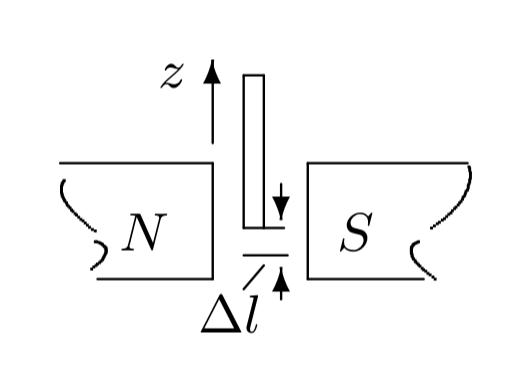
\includegraphics[width=0.3\linewidth]{first}
	\caption{расположение образца в зазоре электромагнита}
\end{figure}

Найдем выражение для магнитной силы, действующей на такой образец (рис. 1). Пусть площадь образца равна $s$, его магнитная проницаемость -- $\mu$, а поле в зазоре равно $B$.
Воспользуемся для расчёта энергетическими соображениями. Магнитная сила может быть вычислена как производная от магнитной энергии по перемещению. Из теории известно, что эту производную следует брать со знаком минус, когда образец находится в поле постоянного магнита, или со знаком плюс, как в нашем случае, когда образец находится в поле в зазоре электромагнита, ток $I$ в обмотках которого поддерживается постоянным.

При смещении образца на $\Delta l$ вниз магнитная сила, действующая на него равна:

\begin{equation}
F = \left( \dfrac{\Delta W_{\text{м}}}{\Delta l}\right)_I,
\end{equation}
где $\Delta W_{m}$ -- изменение магнитной энергии системы при постоянном токе в обмотке электромагнита и, следовательно, при постоянной величине магнитного поля в зазоре.

Магнитная энергия рассчитывается по формуле:

\begin{equation}
W_{m} =  \dfrac{1}{2} \int H B dV = \dfrac{1}{2\mu_0}  \int \dfrac{B^2}{\mu} dV,
\end{equation}
где интеграл распространен на все пространство. При смещении образца, магнитная энергия меняется только в области зазора (в объеме площади $s$ и длины $\Delta l$), около верхнего конца стержня остается неизменной, поскольку магнитного поля там практически нет. Принимая поле внутри стержня равным измеренному нами полю в зазоре $B$ получим

\begin{equation*}
\Delta W_{m} = \dfrac{1}{2\mu_0}\cdot\dfrac{B^2}{\mu}s\Delta l - \dfrac{1}{2\mu_0}\cdot B^2 s\Delta l = \dfrac{1 - \mu}{2\mu_0 \mu}\cdot B^2 s\Delta l = -\dfrac{\chi}{2\mu_0 \mu}\cdot B^2 s\Delta l.
\end{equation*} 
Следовательно, на образец действует сила:

\begin{equation}
F = -\dfrac{\chi}{2\mu_0 \mu}\cdot B^2 s, 
\end{equation}

Знак силы, действующей на образец зависит от знака $\chi$: образцы из парамагнитных материалов ($\chi > 0$) втягиваются в зазор электромагнита, а диамагнетики ($\chi < 0$) выталкиваются из него.

Пренебрегая отличием $\mu$ от единицы, получаем окончательную расчётную формулу в виде

\begin{equation}
F = -\dfrac{\chi B^2 s}{2\mu_0}, 
\end{equation}\

Измерив силу, действующую на образец в магнитном поле $B$ можно рассчитать магнитную восприимчивость образца.

\section*{Экспериментальная установка}
\begin{figure}[!h]
	\centering
	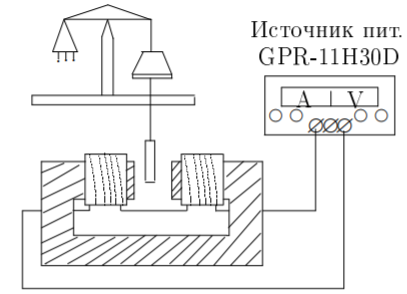
\includegraphics[width = 8cm]{second}
	\caption{Схема экспериментальной установки}
\end{figure}

Схема установки приведена на рис. 2. Магнитное поле с максимальной индукцией $\simeq 1$ Т создается в зазоре электромагнита, питаемого постоянным током. Диаметр полюсов существенно превосходит ширину зазора, поэтому поле в центре зазора достаточно однородно. Величина тока, проходящего через обмотки электромагнита, регулируется при помощи источника питания GPR и измеряется амперметром А, встроенным в источник питания. Градуировка электромагнита (связь между индукцией магнитного поля $B$ в зазоре электромагнита и силой тока $I$ в его обмотках) производится при помощи милливеберметра. 

При измерениях образцы поочередно подвешиваются к аналитическим весам так, что один конец образца оказывался в зазоре, а второй -- вне зазора, где индукцией магнитного поля можно пренебречь. При помощи аналитических весов определяется перегрузка $\Delta P = F$ -- сила, действующая на образец со стороны магнитного поля.

Силы, действующие на диа- и парамагнитные образцы, очень малы. Небольшие примеси ферромагнетиков (сотые доли процента железа или никеля) способны кардинально изменить результат опыта, поэтому образцы были специально отобраны.

\newpage

\section*{Вопросики}

1. Объясните суть метода измерения магнитной восприимчивости.
\vspace{5mm}

Магнитная восприимчивость тел может быть определена через измерение сил, действующих на эти тела в магнитном поле. Существует 2 таких классических метода - это метод Фарадея и метод Гюи. В этой лабе мы пользовались методом Гюи: берётся тонкий длинный стержень, один из концов которого помещается в зазор электромагнита (обычно в область однородного магнитного поля), а другой конец помещается в область пространства, где влиянием магнитного поля можно пренебречь (таким образом, в данном случае закон изменения поля не существенен). Измерив силу, действующую на образец в магнитном поле $B$ можно рассчитать магнитную восприимчивость образца по формуле $F = -\dfrac{\chi B^2 s}{2\mu_0}$

\vspace{5mm}

2. Напишите выражения для магнитной силы, действующей на образец в неоднородном магнитном поле

\vspace{5mm}

$\vec F = (\vec m \nabla)\vec B$

\vspace{5mm}

3. Как можно убедиться в однородности или неоднородности магнитного поля в зазоре электромагнита?

\vspace{5mm}

Если поместить в поле магнитную стрелку, то в случае однородного поля при её перемещении по она будет ориентирована одинаково в силу однородности силовых линий

\vspace{5mm}

4. Как проверить экспериментально, влияет ли намагниченность весов на результаты измерения магнитной восприимчивости?

\vspace{5mm}



\vspace{5mm}

\tbf{5. Принцип работы милливеберметра}
\vspace{5mm}

Милливеберметр М119 принципиально отличается от
обычных приборов магнитоэлектрической системы тем, что на его рамку не действуют упругие
силы, поэтому подвижная система прибора находится в безразличном
равновесии.
В цепь рамки прибора
включается наружная измерительная катушка с известным
числом витков и известной
площадью каждого витка. При
изменении магнитного потока,
пронизывающего измерительную
катушку, в ней возникает ЭДС
индукции и в цепи рамки
милливеберметра течет ток, вызывающий ее поворот и, следовательно, отклонение стрелки
прибора, которое не зависит от ее начального положения и оказывается пропорциональным
изменению магнитного потока. Таким образом, измерение магнитного потока производится по величине максимального отброса стрелки милливеберметра.

\end{document}